\chapter{Spin Analysis}
\label{ch:spin_analysis}
\section{Overview}

The overall goal of this analysis is to arrive at a calculation of our
observable, $A_L$. As discussed in Chapter~\ref{ch:modeling_proton_spin}, $A_L$
is an important probe for the polarized parton distribution functions describing
the quarks and anti-quarks of the proton sea-quark population. There is nothing
magical about $A_L$ - it just so happens that when we construct the asymmetry,
using the cross-sections for a particular process, those cross-sections can be
written in two ways:

\begin{enumerate}
  \item Write it in terms of the machine luminosity and the number of events of
    a particular type observed
  \item Calculate the scattering amplitude for the process, and then the
    cross-section of the process. Write down the cross-section in terms of
    experimental observables.
\end{enumerate}

Thus, our strategy is clear - we have several well established theoretical
frameworks with a number of degrees of freedom (i.e. item 2), so as
experimentalists, we contribute by measuring the cross-section of the
$W\rightarrow\mu$ process, and calculating the observable via the strategy in
item 1, which is then fed back into the models in order to reduce the degrees of
fr and arrive at a more correct model. These models are typically expressed as
global QCD fits to world data over a wide kinematic range, and our contribution
from PHENIX will help constrain the models, therefore giving a more accurate
prediction of how much proton spin we can attribute to coming from the sea-quark
polarization.

The Spin Analysis is very much 'turning the crank', we have already done the
hard part of the analysis in Chapter~\ref{ch:feature_engineering} and
Chapter~\ref{ch:data_wrangling}. Lets not neglect too, the monumental task of
building a RHIC and a PHENIX. The fact that particle physics can even be done
in the first place, is absolutely astounding to me - the amount of
infrastructure, technical expertise, collaboration, financial and intellectual
capital needed to build such an enormous and precise machine is something that
is very difficult to communicate. So, assuming that the other parts of this
massive undertaking have been pulled off without a hitch, the actual machinery
of the Spin Analysis only relies on three items:

\begin{enumerate}
  \item What is the total beam polarization?
  \item What is the polarization of the blue bunch, and yellow bunch at the
    time of each beam-beam interaction which generated a W-genic muon?
  \item What is the total yield of $\mu$'s at forward and backward rapidity,
    for positive and negative charge?
\end{enumerate}

$A_L$ is then calculated:

\begin{equation}
  A_L = {
    {d\sigma^{\Rightarrow} - d\sigma^{\Leftarrow}}
    \over
    {d\sigma^{\Rightarrow} + d\sigma^{\Leftarrow}}
  }
\end{equation}

Where $d\sigma$ is experimentally calculated as:

\begin{equation}
  \sigma = {1\over{\mathcal{L}}}{\dot{N}}
\end{equation}

With $\Rightarrow$ or $\Leftarrow$ referring to tracks which come from
positive($\Rightarrow$) or negative($\Leftarrow$) helicities relative to the
initial proton polarization state. $\mathcal{L}$ refers to the beam luminosity,
a property of the colliding beams, and $\dot{N}$ refers to the production rate
of W-genic muons. Naturally, this calculation is done for forward and backward
rapidities for positive and negative charges. Since we can measure
$W\rightarrow\mu$ for $W+$ or $W-$ at forward or backward rapidities, we treat
everything separately, and combine forward and backward rapidity data to get the
final answer for $A_L^{W+}$ and $A_L^{W-}$ at forward, and backward rapidity.

In practice, we do not calculate cross-sections for $W\rightarrow\mu$ for the
purposes of evaluating $A_L$, as we really only need the yields, since in
principal $\mathcal{L}$ will be a common factor in all cross-sections and cancel
out. This of course comes with major caveats - $\mathcal{L}$ only cancels out if
the relative luminosity of each polarization condition is the same - spin
patterns are chosen so that in theory, this happens. This of course is checked.
Experimentally, we construct raw asymmetries (simple differences/sums) of the
relevant muon yields ($\epsilon_{L}$), and correct the overall raw asymmetry for
less than 100\% beam polarization and the dilution from the signal-to-background
ratio.

\section{Measured Beam Polarization}

Formally, we obtain the beam polarization from the p-Carbon scattering
experiments done every fill, and spin database QA. The polarization of the beams
for each fill are measured at the beginning and end of every fill. This was
described in Section~\ref{sec:beam_polarization}. The results of the
polarization study and spin database QA are all stored in a PostgreSQL database,
indexed by run number (multiple runs are taken in each fill).

The polarization of the blue and yellow beams over the Run 13 run are summarized
in Figure~\ref{fig:avg_polarization}.

\begin{figure}[ht]
  \centering
  \includegraphics[width=\linewidth]{./figures/beam_polarization.pdf}
  \caption{
    Shown: the average beam polarization per run over the course of the 2013
    data set. All of the runs in the analysis were indexed from 0 to
    approximately 1000, and plotted in the order that they were taken. The blue
    open circles are from the blue beam, the yellow open circles are for the
    yellow beam.
  }
  \label{fig:avg_polarization}
\end{figure}

The polarization over the whole of Run 13 was well over 50\% for the majority of
the run, with a few poorly polarized runs. This can be accounted for, by
calculating an asymmetry for every single run, and weighting that asymmetry with
that run's polarization, but it was found that the result was unchanged. This
kind of approach would improve things if the polarization was inconsistent,
though as evident in Figure~\ref{fig:avg_polarization}, it was relatively
consistent (even improving, generally towards the end of the 2013),
distributions of the polarization is summarized in
Figure~\ref{fig:pol_distribution}.

\begin{figure}[H]
	\centering
	\begin{subfigure}[t]{0.5\textwidth}
		\centering
		\includegraphics[width=0.95\linewidth]{./figures/yell_polarization.png}
		\caption{Distribution of Yellow Beam Polarization}
		\label{fig:pol_yell}
	\end{subfigure}%
  \begin{subfigure}[t]{0.5\textwidth}
		\centering
		\includegraphics[width=0.95\linewidth]{./figures/blue_polarization.png}
    \caption{Distribution of Blue Beam Polarization}
		\label{fig:pol_blue}
	\end{subfigure}
	\caption{ 
    The blue beam had a tighter polarization distribution, peaked at just about
    50\% polarization, whereas the yellow beam's polarization distribution was
    broader, still peaking at about 55\%.
  }
	\label{fig:pol_distribution}
\end{figure}

The other major element to the Spin Analysis is determining with what confidence
we can assign to our understanding of the polarization pattern filled into the
blue and yellow beams.

\section{Spin Patterns}

In the 2013 Run Period, I was in charge of the PHENIX spin quality assurance
while the detector was actively taking data. As part of this work it was my job
to maintain the monitoring software as well as confirm that physics fills were
'polarization-ready'. PHENIX uses a numbering system identify which bunch in the
blue beam collides with another bunch from the yellow beam. Blue bunch "0"
collides with yellow bunch "0" at the PHENIX interaction point, by definition.
There are bunches in the blue, and yellow beams which are left purposefully
empty, which allows us to later reconstruct and confirm which bunch is colliding
with which bunch, since if a filled bunch collides with an empty bunch, we will
see no collisions for that event. PHENIX has a slight delay in its triggering
electronics related to the time delay between the DAQ receiving the 'begin run'
event and the first 'data event'. This delay is exactly five bunch-crossings in
length, so when data is reconstructed, recorded bunch crossing numbers in the
data stream will be off by 5. We can look at the BBC rate as a function of bunch
crossing for a data set to identify, and correct this crossing-shift, which is
done in the offline spin data QA.

In the 2013 data taking period, RHIC provided sixteen different bunch patterns -
the patterns were varied to help avoid any kind of systematic bias towards one
bunch polarization over another. For the first half of the 2013 data period,
each beam had two consecutive empty bunches, and a 10-bunch long empty
'abort-gap'. The abort gap is canonically set to occur at bunch number 109-119
(indexing from 0). The consecutive empty bunches occurred at position 68 and 69
in the yellow beam, and 28 and 29 in the blue beam.

Bunch patterns P1-P8 were used in the first half of the data taking period, with
P21-P28 being used in the second half of the data taking period in Run 2013.
Generally, the spin patterns were defined as a sub-pattern, which is then
repeated until the last bunch in a given beam is reached.

\begin{sidewaystable}[ht]
  \centering
  \begin{tabular}{lll}
    \toprule
    \textbf{Pattern} & \textbf{Blue Pattern} & \textbf{Yellow Pattern} \\
    \midrule
    P1  & $++--~++--~++--$             & $++++~----~++++~--$ \\
    P2  & $--++~--++~--++$             & $++++~----~++++~--$ \\
    P3  & $++--~++--~++--$             & $----~++++~----~++$ \\
    P4  & $--++~--++~--++$             & $----~++++~----~++$ \\
    P5  & $++++~----~++++~--$          & $++--~++--~++--$    \\
    P6  & $++++~----~++++~--$          & $--++~--++~--++$    \\
    P7  & $----~++++~----~++$          & $++--~++--~++--$    \\
    P8  & $----~++++~----~++$          & $--++~--++~--++$    \\
    P21 & $++--~++--~++--$             & $--~++++~----~++++~----~++++$ \\
    P22 & $++--~++--~++--$             & $++~----~++++~----~++++~----$ \\
    P23 & $--++~--++~--++$             & $--~++++~----~++++~----~++++$ \\
    P24 & $--++~--++~--++$             & $++~----~++++~----~++++~----$ \\
    P25 & $--~++++~----~++++~----~++++$ & $++--~++--~++--$ \\
    P26 & $--~++++~----~++++~----~++++$ & $--++~--++~--++$ \\
    P27 & $++~----~++++~----~++++~----$ & $++--~++--~++--$ \\
    P28 & $++~----~++++~----~++++~----$ & $--++~--++~--++$ \\
    \bottomrule
  \end{tabular}
  \caption{
    Patters P1-P8 were filled into RHIC for the first portion of the 2013 data
    taking period, with P21-P28 being filling in the second portion. For each
    pattern, from left to right, bunch 0 in the blue or yellow beam is filled
    with the leftmost polarization, with bunch 1 getting the next, and so on.
    The pattern repeats as soon as the end has been reached, until we get to the
    last filled bunch, with any empty bunch being 'polarized' as if it were not
    empty.
  }
  \label{tab:spin_patterns}
\end{sidewaystable}

The patterns are designed to run through as many permutations of bunch-bunch
polarization conditions. The beams are transversely polarized '+' is up and '-'
is down during the fill, but the polarizations are rotated towards PHENIX
(longitudinally) immediately before collision. Crucially, the various collision
conditions need to occur with the same relative frequency - so the patterns are
designed to fulfill this requirement.

Two ways of visualizing the consistency of spin patterns include
Figure~\ref{fig:crossing_count}, which shows, for all muon tracks after the
basic cut, consistent fills. Additionally, if we count the various permutations
of spin patterns, i.e. ++, -+, +-, --, such that the left character is the blue
polarization and the right character is the yellow polarization, we would expect
to see very similar yields for each polarization combination (we do),
Figure~\ref{fig:polarization_counts}.

\begin{figure}
  \centering
  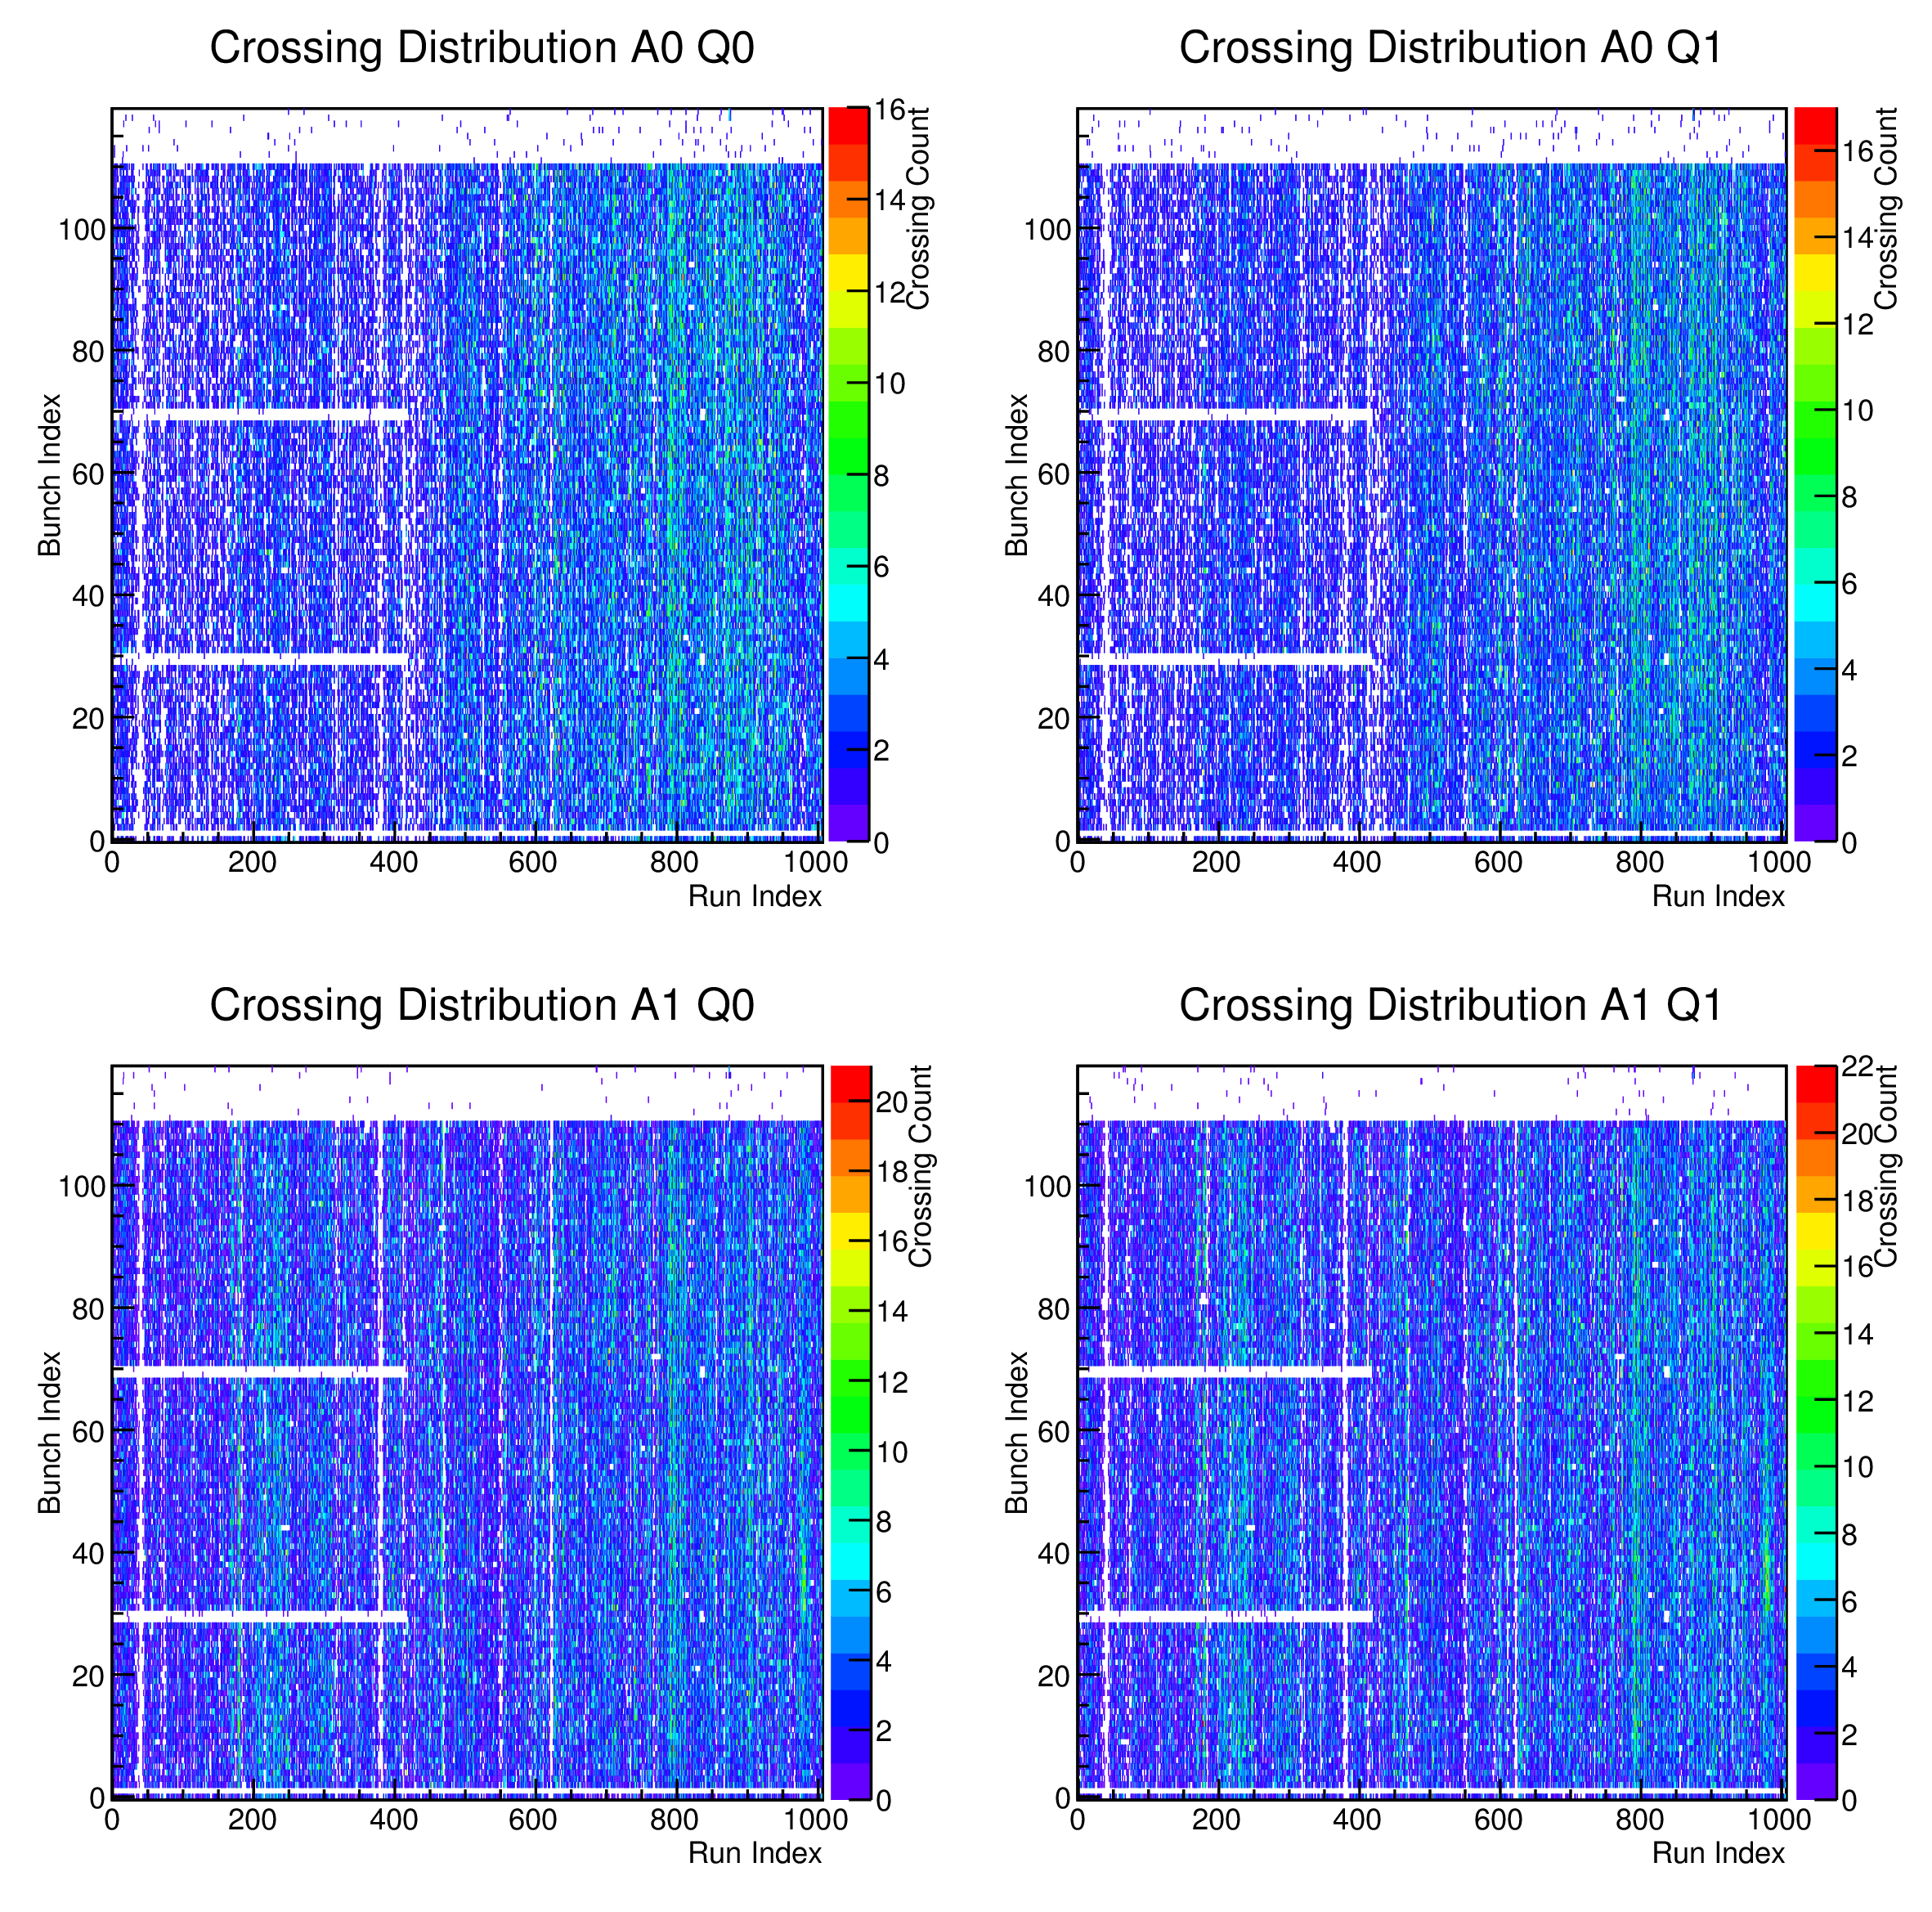
\includegraphics[width=\linewidth]{./figures/crossing_distribution.pdf}
  \caption{
    Here, we see the crossing distribution for every run taken for the 2013 data
    set. We use the typical code for arm/charge. The top row is for the South
    Arm. The Bottom row is for the North Arm. The left column is for negative
    charge, the right column is for positive charge.
  }
  \label{fig:crossing_count}
\end{figure}

\begin{figure}
  \centering
  \includegraphics[width=0.6\linewidth]{./figures/crossing_pattenr_count.pdf}
  \caption{
    Here, we can see the yield for various crossing combinations as taken from
    the dataset itself, rather than the database. We see a very consistent
    distribution between the various possible crossing patterns. In this case,
    the horizontal axis is the crossing pattern code - 0:$++$, 1:$-+$, 2:$+-$,
    3:$--$. Any slight difference between yields for each pattern is well below
    our experimental precision.
  }
  \label{fig:polarization_counts}
\end{figure}

\clearpage
\section{Muon Yields}


\section{Calculation of $A_{L}$ for $W\rightarrow\mu$}
\subsection{Asymmetry Calculation}
\subsection{Discussion of Work Done By Analysis Team}

\section{Data Validation}
Mention Daniel's GPR, Ralf's PEPSI, Abraham's FVTX work, and Francesca's cross-checks.
\subsection{Simulations and The Signal to Background Ratio}
\subsection{Gaussian Process Regression}
\subsection{Four Way Cross Validation}
\subsection{Asymmetry Consistency Check}
\subsection{Beam Polarization}
\subsection{Beam Luminosity}
\subsection{Code Cross Validation}
